\documentclass[a4paper,10pt]{report}
\usepackage{float,graphicx}
\usepackage{amsfonts}
\usepackage{amsthm}
\usepackage{amsmath}
\usepackage{amssymb}
\usepackage{wrapfig}
\usepackage{minted}
\usepackage{mathrsfs}
\usepackage{pgfplots}
\usepackage{mdframed}
\usepackage{multirow}
\usepackage[lined,boxruled]{algorithm2e}\usepackage{color}
\usepackage[english]{babel}

\newcommand{\ac}[1]{\textcolor{red}{AC: #1}}
\newcommand{\af}[1]{\textcolor{blue}{AF: #1}}

\pgfplotsset{width=10cm,compat=1.9}
\usemintedstyle{friendly}
\BeforeBeginEnvironment{minted}{\begin{mdframed}}
\AfterEndEnvironment{minted}{\end{mdframed}}
\begin{document}
\title{\Large{\textbf{Inducing game rules from varying quality game play}}}
% \title{\Large{\textbf{Inductive general game playing with varying quality game play}}}
\author{Alastair Flynn}
\maketitle

\begin{abstract}

General Game Playing (GGP) is a framework in which an artificial intelligence program is required to play a variety of games successfully. It acts as a test bed for AI and motivator of research. The AI is given a random game description at runtime (such as \textit{checkers} or \textit{tic tac toe}) which it then plays.
The framework includes repositories of game rules written in a logic programming language.


The Inductive General Game Playing (IGGP) problem challenges machine learning systems to learn these GGP game rules by watching the game being played. In other words, IGGP is the problem of inducing general game rules from specific game observations. Inductive Logic Programming (ILP), a subfield of ML, has shown to be a promising approach to this problem though it has been demonstrated that it is still a hard problem for ILP systems.

Existing work on IGGP has always assumed that the game player being observed makes random moves. This is not representative of how a human learns to play a game, to learn to play chess we watch someone who is playing to win. With random gameplay situations that would normally be encountered when humans play are not present. Some games rules may not come into effect unless the game gets to a certain state such as \textit{castling} in \textit{checkers}.

To address this limitation, we analyse the effect of using intelligent versus random gameplay traces as well as the effect of varying the number of traces in the training set.

We use Sancho, the 2014 GGP competition winner, to generate intelligent game traces for a large number of games. We then use the ILP systems, Metagol, Aleph and ILASP to induce game rules from the traces.
We train and test the systems on combinations of intelligent and random data including a mixture of both. We also vary the volume of training data.

Our results show that whilst some games were learned more effectively in some of the experiments than others no overall trend was statistically significant.

The implications of this work are that varying the quality of training data as described in this paper has strong effects on the accuracy of the learned game rules; however one solution does not work for all games.




% When learning programs in Inductive Logic Programming (ILP) optimisations to the dataset used to train the systems can often be as effective as improvements to the systems themselves.


\end{abstract}

\chapter{Introduction}
General Game Playing (GGP) is a framework in which artificial intelligence programs are required to play a large number of games successfully.\cite{Genesereth/GGPOverview}. Traditional game playing AI has focused on a single game. Famouse AI such as IBMs deep blue is able to beat grand masters at chess but is completetly unable to play checkers \ac{citation needed}. These traditional AI also only do part of the work. A lot of the analysis of the game is done outside of the system. A more interesting challenge is building AI that can play games without any prior knowlegde. In GGP the AI are given the description of the rules of a game at runtime. Games in the framework range greatly in both number of players and complexity; from the single player Eight Puzzle to the six player Chinese Checkers, and from the relativly simple Rock Paper Scissors to Chess\cite{GGP-Website}. The progress in the field is consolidated annually at the GGP where participants compete to find the best GGP AI.

The GGP framework includes a large database of games. In a GGP match games from these databases are selected at random and sent to the competitors. The games are specified in the Game Description Language (GDL), a logic programming language built for describing games as state machines\cite{GDL_Spec}. A logic programming language being any that is mainly based on formal logic, such as Prolog.


\begin{figure}[ht]
	\centering
	\fbox{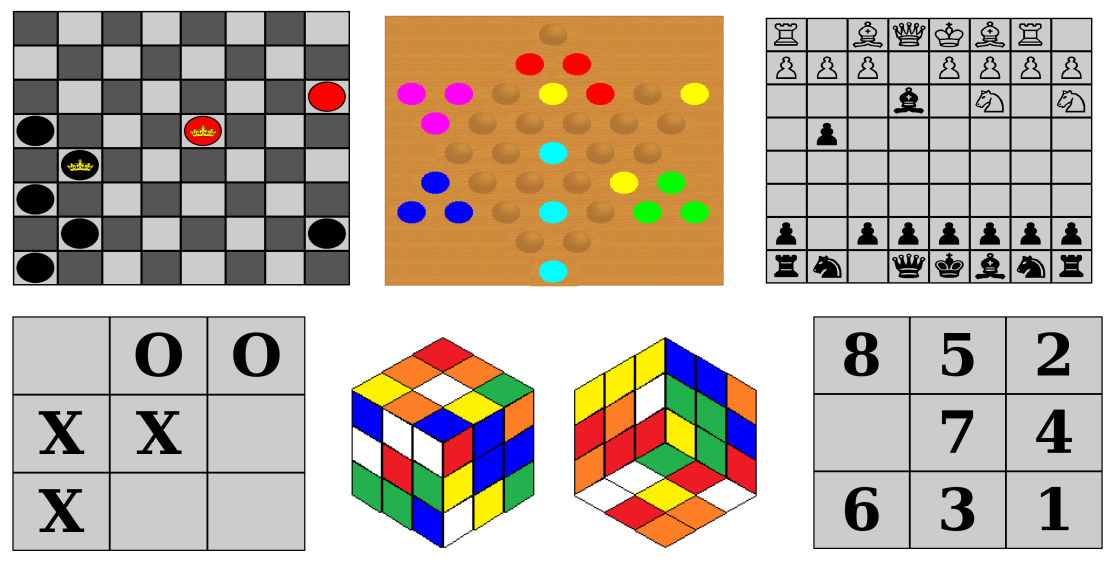
\includegraphics[width=0.7\linewidth]{GGP-Games.png}}
	\caption{A selection of games from the GGP competition. From the top right: \textit{checkers}, \textit{chinese checkers}, \textit{chess}, \textit{tic tac toe}, \textit{rubix cube} and \textit{eight puzzle}}
\end{figure}

\begin{listing}[ht]
\begin{minted}[fontsize=\footnotesize]{text}
(succ 0  1)
(succ 1  2)
(succ 2  3)
(beats scissors paper)
(beats paper stone)
(beats stone scissors)
(<= (legal ?p scissors) (player ?p))
(<= (legal ?p paper) (player ?p))
(<= (legal ?p stone) (player ?p))
(<= (draws ?p) (does ?p ?a) (does ?q ?a) (distinct ?p ?q))
(<= (wins ?p) (does ?p ?a1) (does ?q ?a2) (distinct ?p ?q) (beats ?a1 ?a2))
(<= (loses ?p) (does ?p ?a1) (does ?q ?a2) (distinct ?p ?q) (beats ?a2 ?a1))
\end{minted}
\caption{
\ac{is this listing referenced in the text?}
A sample of rules from the GDL description of Rock Paper Scissors. The $?$ indicates a variable and $<=$ indicates an implication with the first expression after being the head and the conjugation of the rest making up the body
}
\end{listing}


These GDL game descriptions form the basis for the Inductive General Game Playing (IGGP) problem \ac{citation needed}. The task is an inversion of the GGP problem. Rather than taking game rules and using them to play the game in IGGP the aim is to learn the rules from observations of gameplay, similar to how a human might work out the rules of a game by watching someone play it. Cropper et al. define the IGGP problem in their 2019 paper; given a set of gameplay observations the goal is to induce the rules of the game\cite{Cropper/IGGP}. The games used in IGGP are those from the GGP competition problem set, specified in GDL, meaning they are widely varied in complexity.

\af{GIVE EXAMPLE OF IGGP PROBLEM}

An effective way of solving the IGGP problem is a form of machine learning: Inductive Logic Programming (ILP) \ac{citation needed}. In ILP, the learner is tasked with learning logic programs given some background knowledge and a set of values for which the programs are true or false (also expressed in a logical programming language). In the IGGP paper \cite{Cropper/IGGP}, the authors showed through empirical evaluations that ILP systems achieve the best score in this task compared to other machine learning techniques. The ILP system derive a hypothesis, a logic program that when combined with the background knowledge, entails all of the positive and none of the negative examples\cite{Muggleton/ILP}. In the IGGP paper\cite{Cropper/IGGP} it is also shown that the problem is hard for current ILP systems, with on average only 40\% of the rules being learned by the best performing systems.

However, the existing work has limitations. All existing work has assumed that the gameplay being observed is randomly generated. Rather than agents playing to win they simply make moves at random. Often this has the result of the game terminating before it reaches a terminal state due to a cap on trace length or sections of the rule set remaining completely unused. In previous work there has also not been any research done to ascertain the effects that increasing the number of game observation has on the quality of the induced rules. It is unknown weather there is a threshold at which new any new game traces introduced are insignificant. In this paper we use the IGGP framework to evaluate the ability of ILP agents to correctly induce the rules of a game given different sets of gameplay observations - optimal gameplay verses random gameplay as well as combinations of the two. We also vary the number of gameplay traces from which the ILP systems learn.


It is not obvious whether random or optimal gameplay would be best. When learning the rules of chess would a human rather watch moves being made randomly, or a match between two grandmasters? It is not an easy question to answer. Both situations will result in a restricted view of the game, with certain situations never occurring in each one. This is not only a dilemma in the context of learning game rules. For example, teaching a self driving car to navigate roads requires training it on examples of driving. We would clearly not train it on optimal Formula One quality driving and neither would we train it on random movement of the car. The question to be asked is what is the ideal level of training data to use to best teach a system the rules you want it to learn. In this paper, we try to help give some insight into this fundamental question. Specifically, we ask the following research questions:

\begin{description}
\item[Q1] Does varying the quality of game traces influence the ability for learners to solve the IGGP problems? Specifically, does the quality of game play affect predictive accuracy?
\item[Q2] Does varying the amount of game traces influence the ability for learners to solve the IGGP problems? Specifically, does the quality of game play affect predictive accuracy?
\item[Q3] Can we improve the performance of a learner by mixing the quality of traces?
\end{description}

We will train a range of ILP systems that each use a different approach to the problem on different sets of training data. The results for Q1 will be the most interesting as it is not clear what the expected outcome is. Q2 is an \aco{easier}{probably a better word than easier} question to answer, it is generally accepted that for machine learning problems the more training data you have the better the predictive accuracy of the ML system \ac{citation needed}. We ask this question to get some insight into how much the predictive accuracy is affected by the training set size. Often in ILP only a small amount of training data is needed, adding more data may not significantly affect accuracy \cite{Muggleton/ILP}. The third question is an interesting one. Intuitively greater diversity in the training data should give a result closer to the rule that generated the data. However if a learner is trained on random data and only tested on random data we would expect this to perform better than a learner trained on random data then tested on a mix of optimal and random data. This question thus highlights an issue we face: how do we test the learned game rules?

Ideally the generated rules would be compared directly against the rules in the GDL game descriptions. We would take the generated rule and see for what percentage of all possible game states the reference rule and the learned rule gave the same output. Unfortunately we do not have the computational resources to do this with a lot of the games having too many possible states such as checkers which has a state-space complexity of roughly $5.0 \cdot 10^{20}$\cite{Horssen/Checkers} and sudoku which exceeds $6.6 \cdot 10^{21}$\cite{Felgenhauer/Suduko}. Instead we will test the learned programs on both optimal and random data of the same quality used in training. \af{and maybe a combination as well}

We would also expect models trained on the same distribution as they are tested on to perform best since it is generally accepted that the accuracy of a model increases the closer the test data distribution is to the training data distribution \cite{Mitchell/MachineLearing}. However, Gonzales and Abu-Mostafa\cite{Gonzalez/MismatchedOutperform} suggest that a system trained on a different domain to the one it is tested can outperform a system trained and tested on the same domain. Given a test distribution there exsists a duel distribution that, when used to train, gives better results. The duel distribution gives a lower out-of-sample\footnote{out-of-sample data is data that is not in the training set} error than using the test distribution. This duel distribution can be thought of as the point in the input space where the least out-of-sample error occurs\cite{Gonzalez/MismatchedOutperform}. As well as optimising the single training distribution we can take data from multiple distinct distributions. Ben-David et. al. show that training data taken from multiple different domains can in fact give lower error on testing data that traning data taken from any single domain, including the testing domain \cite{Ben-David/DifferentDomains}. It is not clear in our case what selection of training data will result in the most effect learning.

To help answer questions 1-3, we make the following contributions:

\subsubsection{Contributions}
\begin{itemize}
\item We implement a system to play GGP games at (1) random, \af{(2) world-leading}, and (3) optimal levels. (Section \ref{sec:experiments})
\item We transform the GGP traces to IGGP problems
\item We train the ILP systems Metagol, Aleph and ILASP on different combinations of optimal and random data as well as testing them on each individually (Section \ref{sec:experiments})
\item We train the ILP systems on differing amounts of traces and test to ascertain the effect this has on the accuracy of the predicted results
\end{itemize}
\chapter{Related work}

\section{GGP}

General game playing is a framework for evaluating an agenet's general intelligence accross a wide range of tasks \cite{Cropper/IGGP}. The idea is that agents are able to accept declarative descriptions of arbitrary games at run time and are able to use such descriptions to play those games effectively. All the games are finite, discrete, deterministic multi-player games of complete information. The games also vary in number of players, dimensions and complexy. For example games such as rock paper scissons have 0 dimensions and only 10 rules in the given GGP ruleset, more complex games such as checkers has 52 rules and are 2 dimensional. There are also single player games such as Eight Puzzle or Fizz Buzz.

The agents play games selected at random. They are send a listing of the rules descirbed in the Game Description Language (GDL). GDL is a language based on first order logic described in section \ref{sec:GDL}. The list of games along with their descriptions are available online \footnote{http://ggp.stanford.edu/iggpc/ accessed on 17/03/2020}. Matches in the GGP framework take place through an online framework called the Gamemaster. The agents connect to an online Game Manager (part of the Gamemaster) service which arbitrates indavidual matches. The connecting agents send several pieces of information to the Game Manger incliding a game that is already know by the manager and the required number of players. The match can then be started by pressing a start button, when pressed the agents will recive a \textit{Start} message including the role of the player (e.g. black or white in chess) and a description on the game in GDL. The Game Manger communicates all instructions to the players through HTTP\cite{Genesereth/GGPOverview}.

In 2005 an annual International General Game Playing Competition (IGGPC) was set up which still runs to this day\cite{Kowalski/GGP}. Each year hopeful participants pit GGP agents against one another to determine the most effective system. The competitors take part in a series of rounds of increasing complexity. The agent that wins the most games in these rounds is declared victorious. The 2014 winner Sancho is used in this paper to generate optimal game traces for the IGGP task. The game descriptions written in GDL used in the GGP competition can be used as ideal rule sets for systems in Inductive General Game Playing (IGGP) to generate. The descriptions of the games used in GGP are not necessarily minimal so it is possible that an ILP system could generate a more concise ruleset the the GGP descriptions.

\subsection{GDL}\label{sec:GDL}
Game definition language is the formal language used in the GGP competition to specify the rules of the games.\cite{GDL_Spec} The language is based off logical programming languages such as Prolog and is in fact a logical programming language itself.
\subsubsection{Logical Programming}
Logic programming is a programming paradigm based on formal logic. Programs are made up of facts and rules. Rules are made up of two parts: the head and the body. They can be read as logical implications where the conjunction of all the elements in the body imply the head. The syntax is different for different logical programming languages but the head is usually written before the body. A fact is simply a rule without a body, that is, a statement that is taken as true. The compiler takes queries and returns weather they are true of false. If there are free variables in the query the compiler assigns them values for which the query is true. Logical programming is good for symbolic non-numeric computation. It is well suited to solving problems that involve well defined objects and relations between them, such as a GGP game.
\subsubsection{Usefulness of GDL}
The game description language was designed specifically to represent finite, discrete, deterministic multi-player games of complete information. It is suited to specifying game rules because:
\begin{itemize}
\item It is a purely declarative language
\item It has restrictions to ensure that all questions of logical entailment are decidable
\item There are some reserved words (such as \textit{terminal} or \textit{goal}), which tailor the language to the task of defining games
\end{itemize}
These descriptions define the games in terms of a set of true facts capturing the information needed to give the following predicates:
\begin{itemize}
\item The initial game state
\item The goal state
\item The terminal state
\end{itemize}
In addition, logical rules are used to describe the following:
\begin{itemize}
\item The legal moves for a given player and state
\item The next state for a given player state and move
\item The termination and goal conditions
\end{itemize}
In the IGGP problem the given task is to generate the rules for the goal, the next state, the legal states and the terminal state.
%more examples?

\section{Prolog}
Prolog is one of the most popular and well used logical programming languages. The syntax in Prolog for rules and facts is fairly intuitive. A simple fact might be \mintinline{Prolog}{son(bob,alice).}. This tells us that the atom \mintinline{Prolog}{alice} relates the atom \mintinline{Prolog}{bob} in the \mintinline{Prolog}{son} relation. A rule is written \mintinline{Prolog}{parent(X,Y) :- son(Y,X)} which means if we have the relation son of Y and X then X relates Y in parent. The symbol :- is the same as reverse implication ($\Leftarrow$). We can query a program in the Prolog environment. If we typed in "\mintinline{Prolog}{parent(alice,bob).}" then it would return true because we have \mintinline{Prolog}{son(bob,alice)} and the rule which tells us that if X is a son of Y else then Y is a parent of X so \mintinline{Prolog}{alice} is a parent of \mintinline{Prolog}{bob}. Predicates can be conjoined with the comma "," (e.g. \mintinline{Prolog}{a(X,Y,Z) :- b(X,Y), c(Z,Y)}). Disjunction is expressed with the semicolon ";" (e.g. \mintinline{Prolog}{a(X,Y,Z) :- b(X,Y) ; c(Z,Y)}.

Prolog answers queries using a process know as proof seach and unification. The unification process is similar to logical unification, two terms unify if they are the same term or if they contain variables that can be instantiated with terms in such a way that the new terms are equal. For example the terms \mintinline{Prolog}{name(bob).} and \mintinline{Prolog}{name(X).} will unify with \mintinline{Prolog}{X = bob}. The Prolog ISO defines the Herbrand Algorithm for unification \cite{PrologISO}. A Prolog query is a set of goals. The Prolog System decides weather they are satisfiable or not. When a query is asked the of the Prolog system it executes something similar to the following algorithm. The exact implementations vary among Prolog systems however they are all roughly this algorithm.
\begin{algorithm}
\SetKwInOut{Input}{Input}
\SetKwProg{Fn}{Function}{}{}
\Input{A list of goals $GoalList = G_1,G_2,...,G_M$}
\Fn{\textbf{execute} (Program, GoalList, Success):}{
    \If{$empty(GoalList)$}{$Success \leftarrow true$}{
        \While{\textbf{not} empty($GoalList$)}{
            $\textit{Goal} \leftarrow head(GoalList)$\;
            $OtherGoals \leftarrow tail(GoalList)$\;
            $Satisfied \leftarrow false$\;
            \While{\textbf{not} Satisfied and there are more clauses in the program}{
                Let next clause in the program be $H \vdash B_1,...,B_n$\;
                Construct a variant of this clause $H' \vdash B_1',...,B_n'$\;
                $match(Goal,H',MatchOK,Instant)$\;
                \If{$MatchOK$}{
                    $NewGoals \leftarrow append([B_1',...,B_n'],OtherGoals)$\;
                    $NewGoals \leftarrow substitue(Instant,NewGoals)$\;
                    $execute(Program,NewGoals,$\textit{Satisfied}$)$\;
                }
            }
        $Success \leftarrow$ \textit{Satisfied};\;
        }
    }
}
\caption{Execute Prolog Goals}
\end{algorithm}

the program listing is wearched for a term to unify with. The listing is searched in the order it is written in. When Prolog finds a matching rule it then attempts to sequentially unify the terms of the body using the same method. If the rule has no body then the variables are assigned and the terms unify. If Prolog fails to unify two terms then it backtracks, assignes the last variable a differnt values. This continues until a proof is found or all possibilities have been exauseted\cite{Bratko}.


\section{IGGP}
The Inductive General Game Playing (IGGP) problem is an inversion of the GGP problem. Rather than using game rules to generate gameplay the learner must learn the rules of the game by watching others play. The learner is given a set of game traces and is tasked with using them to induce (learn) the rules of the game that could have produced the traces\cite{Cropper/IGGP}. IGGP was designed as a way of benchmarking machine learning systems.

The definition of task itself is based on the Inductive logic programming problem.

\subsection{ILP}\label{sec:ILP}
Inductive logic programming is a form of machine learning that uses logic programming to represent examples, background knowledge, and learned programs\cite{Cropper/EfficientLearning}. To learn the program is supplied with positive examples, negative examples and the background knowledge. In the general inductive setting we are provided with three languages.
\begin{itemize}
\item $\mathcal{L}_O$: the language of observations (positive and negative examples)
\item $\mathcal{L}_B$: the language of background knowledge
\item $\mathcal{L}_H$: the language of hypotheses
\end{itemize}
The general inductive problem is as follows: given a consistent set of examples or observations $O \subseteq \mathcal{L}_O$ and consistent background knowledge $B \subseteq \mathcal{L}_B$ find an hypothesis $H \in \mathcal{L}_H$ such that \[B \wedge H \vDash O\] \cite{Muggleton/ILP}
That is that the generated hypothesis and the background knowledge imply the positive examples and not imply the negative examples.

\af{Example task (grandparent relation)}

ILP systems generally regard ILP as a search problem. The search space is the set of well formed hypothesis. Often a set of inference rules are applied to the starting hypothesis, the new hypothesise are then pruned and expanded according to how often $B \wedge H \vDash O$ in the observations $O$. When all the observations are implied then a correct program has been found.

\subsection{Back to IGGP}

In IGGP we also have the idea of background knowledge and positive or negative observations. The task is given as a triple $\{(B,E^+,E^-)\}$. The positive examples $E^+$, the negative examples  $E^-$ and the background knowledge $B$. Similar to the Inductive logic programming problem the learner \ref{sec:ILP} has to come up with a hypothesis $H$ such that $H$ and the background knowledge imply all the positive examples but none of the negative examples, that is $H \cup B \models E^+$ and $H \cup B \not\models E_i^-$. All three are given in the form of a set of ground atoms, that is they do not contain any free variables.The background knowledge of a task consists of all the rules of the GDL game description that do not concern the predicate being learned. For example in Rock Paper Scissors this would be the facts that give which item beats which (i.e. that scissors beat paper). An example of a typical IGGP problem is given below

%Show example IGGP task

The IGGP problem itself is described in section \ref{sec:LogicalSetting}.

The IGGP dataset, also given in the same paper as the definition of the problem. It is a collection of 50 games, specified in GDL. The purpose of this database is to standardises the set of games used in the IGGP problem to allow for results to be easily compared. It is in fact the set of games that this paper is based on.
A mechanism is also provided by the authors to turn these GDL game descriptions in the set into new IGGP tasks. This method plays the games randomly to generate the observations. In this paper we modify the mechanism to generate optimal game traces.











%To evaluate ILP systems the learning tasks they are given need to be small enough that it is feasible for them to learn the programs, but also diverse enough that we test the full capability of the system. The Inductive general game playing framework provides this. To understand IGGP we first need to explain the General game playing framework.





% \chapter{ILP systems}
\section{ILP systems used}
We use three ILP systems to compare the effects of different learning data, Metagol, Aleph and ILASP. All three systems use different approaches the ILP problem.
\subsection{Metagol}
The Metagol ILP system is a meta-interpreter for Prolog, that is, it is written in the same language is evaluates. Metagol takes positive and negative examples, background knowledge and meta-rules. Meta rules are specific to Metagol. They determin the shape of the induced rules and are used to guide the search for a hypothesis. An example of a metarule is the \texttt{chain} rule \[P(A,B) \leftarrow Q(A,C),R(C,B)\] The letters P, Q and R represent existentially quantified second order variables, A, B and C are regular Prolog variables. When trying to induce rules the second order variables are substituted for predicates from the background knowledge or the hypothesis itself. To illustrate this consider a metarule being applied when learning the predicate \textit{last(A,B)} where a is a list and b is the last element in it. Given the positive example
\begin{minted}{Prolog}
last([a,l,g,o,r,i,t,h,m],m).
\end{minted}

As well as the background predicates \textit{reverse/2} and \textit{head/2} the chain rule might be used to derive the rule
\begin{minted}{Prolog}
last(A,B) :- reverse(A,C), head(C,B)
\end{minted}


\cite{Andrew/ILP-review}\cite{Rolf/Metagol}\cite{Metagol/Github}
\begin{enumerate}
\item Select a positive example (an atom) to generalise. If none exists, stop, otherwise proceed to the next step.
\item Try to prove an atom using background knowledge by delegating the proof to Prolog. If successful, go to step 1, otherwise proceed to the next step.
\item Try to unify the atom with the head of a metarule and either choose predicates from the background knowledge that imply the head to fill the body. Try proving the body predicate, if it cannot be proved try different BK\footnote{To prove the body predicate the whole procedure is called again with the body predicates as the positive examples. For example if we had \texttt{last([a,b],b)} as our positive example and have tried to use the chain metarule to with reverse and head we would then call the whole procedure again with the positive examples as [reverse([a,b], C),head(C,b)] if this was successful then we continue, otherwise we try different predicates}. If no BK can be found that prove the positive example then try adding a new invented predicate and attempt to prove this\footnote{For example we might replace head with an invented predicate in the previous footnote example}.
\item Once you find a metarule substitution that works add it to the program and move to the next atom
\end{enumerate}


The end hypothesis is all the metarule substitutions. It is the checked that the negative atoms are not implied by the hypothesis, if they are a new one is generated. When the hypothesis is combined with the background knowledge the positive examples, but not the negative examples, are implied.

The choice of metarules determines the structure of the hypothesis. Different choice of metarules will allow different hypotheses to be generated. Deciding which metarules to use for a given task is an unsolved problem \cite{Cropper/Thesis}. For this task a set of 9 derivationally irreducible metarules are used which remain consistent across all tasks.
\subsection{ALEPH}
Aleph is an Prolog variant of the ILP system Progol \cite{Muggleton/Aleph}. As input, like any other ILP system, Aleph takes positive and negative examples represented as a set of facts along with the background knowledge. It also requires \textit{mode declarations} and \textit{determinations} which are specific to Aleph. Mode declarations specify the type of the inputs and outputs of each predicate used e.g. \texttt{plus(+integer,+integer,-integer)} where \texttt{+} signifies an input and \texttt{-} an output.
Determinations specify which predicates can go in the body of a hypothesis. These determinations take the form of pairs of predicates, the first being the head of the clause and the second a predicate that can appear in its body.

For each predicate we would like to learn in the IGGP problem we give Aleph the determinations consisting of every target predicate (next,goal and legal) paired with every background predicate (which are specific to each game). Luckily there has been some work to induce mode declarations from the determinations \cite{McCreath/Meta-extraction} so we do not need to come up with our own mode declarations.

A basic outline of the Aleph algorithm is taken from the aleph website \footnote{http://www.cs.ox.ac.uk/activities/programinduction/Aleph/aleph.html accessed 26/03/2020}:
\begin{enumerate}
\item Select an example to be generalised. If none exist, stop, otherwise proceed to the
next step.
\item Construct the most specific clause (also known as the bottom clause \cite{Muggleton/Aleph}) that entails
the example selected and is within language restrictions provided.
\item Search for a clause more general than the bottom clause. This step is done by search-
ing for some subset of the literals in the bottom clause that has the 'best' score.
\item The clause with the best score is added to the current theory and all the examples
made redundant are removed. Return to step 1.
\end{enumerate}

Mode declarations and determinations are used in step 2 of this procedure to bound the hypothesis space. Only predicates that are mentioned in the determinations of the hypothesis and are of the correct type are tried. The bottom clause constructed is the most specific clause that entails the example. Therefore a clause with the same head and any subset of the predicates of the body will be more general than the bottom clause. Aleph only considers these generalisations of this bottom clause. The search space is therefore bounded by $2^n$ with $n$ being the number of predicates in the bottom clause.

By default Aleph preforms a bounded breath first search on all the possible rules, enumerating shorter clauses before longer clauses. The search is bounded by several parameters such as maximum clause size and maximum proof depth. The best score is selected as the one with the best $P - N$ value where $P$ is the number of positive rules entailed by the hypothesis and $N$ is the number of negative rules entailed. For this paper we will use Aleph with the default settings.

\subsection{ILASP}

ILASP is an ILP system based on Answer Set Programming (ASP). An introduction to ASP can be found here \cite{Corapi/ASP}. ILASP uses a subset of ASP that is defined in these papers\cite{ILASP-Manuel}\cite{MarkLaw/OG-ILASP}\cite{MarkLaw/Thesis} The ILASP process effectively generates all possible rules of a certain length, turns the problem into an ASP problem that adds a predicate to each rule allowing it to be active or inactive. It then uses the ASP solver clingo\cite{Clingo}  to check which rules should be active if the program is to be consistent with the positive and the negation of the negative examples\cite{MarkLaw/OG-ILASP}\cite{MarkLaw/Thesis}. In this paper we use a version of ILASP based on ILASP2i\cite{MarkLaw/ILASP2i} which was developed with the IGGP problem in mind\cite{Cropper/IGGP}. As one input ILASP takes a hypothesis search space, i.e. the set of all hypotheses to be considered. This is constructed using the type signatures given for each problem that are provided in the IGGP dataset.

An ILASP task is defined as a tuple $T = \langle B,S_M,E^+E^-\rangle$ where $B$ is the background knowledge, $S_M$ is the hypothesis space, and $E^+$ and $E^-$ are the positive and negative examples. The ILASP procedure is given in algorithm \ref{alg:ILASP}.
\begin{algorithm}[H]\label{alg:ILASP}
    \SetAlgoLined
    $n$ = 0\;
    solutions = []\;
    \While{solutions.empty}{
        $S^N$ = all possible hypotheses of length $N$ from $S_M$ \;
        $ns$ = all subsets of $S^N$ that imply $E^-$ (Using an ASP solver)\;
        $vs$ = the set of rules that for each set of rules in $ns$ imply false if exactly those rules are active\;
        solutions = all subsets of $S^N$ that imply $E^+$ and satisfy $vs$ (using asp solver)\;
        $n$ = $n$ + 1\;
    }
    \caption{ILASP outline}
\end{algorithm}

The approaches used by ILASP have proved to be well suited to the IGGP task \cite{Cropper/IGGP}. We expect it to do well in the experiments conducted.
% \chapter{Logical setting}
\chapter{IGGP problem}
\label{ch:IGGP}

The IGGP problem is defined in the 2019 paper Inductive General Game Playing \cite{Cropper/IGGP}. Much like the problem of ILP described in section \ref{sec:ILP} the problem setting consists of examples about the truth or falsity of a formula $F$ and a hypothesis $H$ which covers $F$ if $H$ entails $F$. We assume the languages of:
\begin{itemize}
\item $\mathscr{E}$ the language of examples (observations)
\item $\mathscr{B}$ the language of background knowledge
\item $\mathscr{H}$ the language of hypotheses
\end{itemize} 
Each of these languages can be see as a subset of those described in \ref{sec:ILP}. These languages are made up only of function free ground atoms. In our experiments we transform data from the GDL descriptions of games in the IGGP dataset and transform it into the languages of $\mathscr{B}$ and $\mathscr{E}$. GDL allows for functions (predicates nested in one another) in rules albeit in a restricted form. For example any atom appearing inside a \texttt{true} predicate such as \texttt{true(count(9))}. We flatten all of these to single, non nested predicates, i.e. \verb|true_count(9)|. This is needed as not all ILP systems support function symbols. We can therefore assume that both $\mathscr{E}$ and $\mathscr{B}$ are function-free. The language of hypotheses $\mathscr{H}$ can be assumed to consist of datalog programs with stratified negation as described here\cite{Kenneth}. Stratified negation is not necessary but in practice allows significantly more concise programs, and thus often makes the learning task computationally easier. We first define an IGGP \textit{input} then use it to define the IGGP \textit{problem}. The IGGP input needs to capture the idea of a set of observations about a game. The input is based on the general input for the Logical induction problem of section \ref{sec:ILP} since this is a sub problem of it.

\textbf{The IGGP Input:} An input $\Delta$ is a set of triples $\{(B_i,E_i^+,E_i^-)\}_m^{i=1}$ where
\begin{itemize}
\item $B_i \subset \mathscr{B}$ represents background knowledge
\item $E_i^+ \subseteq \mathscr{E}$ and $E_i^- \subseteq \mathscr{E}$ represent positive and negative examples respectively
\end{itemize}
The IGGP input composes the IGGP problem as follows:

\textbf{The IGGP Problem:} Given an IGGP input $\Delta$, the IGGP problem is to return a hypothesis $H \in \mathscr{H}$ such that for all $(B_i,E_i^+,E_i^-) \in \Delta$ it holds that $H \cup B_i \models E_i^+$ and
$H \cup B_i \not\models E_i^-$.


\subsubsection{Problem Setting}
\af{this section probably needs improving}

Let the accuracy of a set $I$ of ILP systems be defined as the mean of the percentage accuracy of each of them when tested on a given set of examples.

Given an set of ILP systems $I$, for what selection of game traces $\Delta$ combined from an optimal gameplay distribution and a random gameplay distribution are the systems most accurate when solving the IGGP problem. The accuracy of $I$ when solving the IGGP problem will be tested by evaluating each $i \in I$ with data taken from a 50/50 combination of both optimal and random distributions.

Also given a set of ILP systems $I$, and a gameplay distribution $G$ how does the number of training samples $|\Delta|$ taken from $G$ affect the accuracy of the hypothesis $H$ for each $i \in I$ when tested on $G$.


\chapter{Systems used}
\section{Generating Traces}
\subsection{Sancho}
To generate optimal gameplay we decided that the best approach was to use a previous winner of the GGP competition. Since the aim of the competition is to find the program that performs best at the set of games used in the IGGP problem we conclude that there is no better way to generate a comprehensive set of game traces. The winner of the 2014 GGP competition 'Sancho' was selected \footnote{http://ggp.stanford.edu/iggpc/winners.php accessed on 12/03/2020} since they are the most recent winner to have published their code \footnote{http://sanchoggp.github.io/sancho-ggp/ access 12/03/2020}. Some small modifications to the information logged by the game server are made but otherwise the code is unchanged.

The core of Sancho is the Monte Carlo tree search (MCTS) algorithm.

\subsubsection{Monte Carlo Tree Search}
Given a game state the basic MCTS will return the most promising next move. The algorithm achives this by simulating random playouts of the game many times. The technique was developed for computer Go but has since been applied to play a wide range of games effectively including board games and video games\cite{Silver/MCTS}\cite{Chaslot/MCTS}.

The use of random simulation to evaluate game states is a powerful tool. Information about the game such as heuristics for evaluating non terminal states are not needed at all, the rules of the game are enough on their own. In the case of the GGP problem this is ideal. The rules of the game are only revealed shortly before the game is played meaning deriving effective heuristics is a hard problem.

In our case all games being played are sequential, finite and discrete so we only need to consider MCTS for this case.
% say why it is good for this

% possibly put in a diagram of game tree
The MCTS is a tree search algorithm, the tree being searched is the game tree. A game tree being a tree made up of nodes representing states of the game and the children of each node being all the states that can be moved to from that state. The leaves of this tree are the terminal states. The search is a sequence of traversals of the game tree. A traversal is a path that starts at the root node and continues down until it reaches a node that has at least one unvisited child. One of these unvisited children are then chosen to be the start state for a simulation of the rest of the game. The simulation chooses random moves, playing the game out to a terminal state. The result of the simulation is propagated back from the node it started at all the way to the root node to update statistics attached to each node. These statistics are used to choose future paths to traverse so more promising moves are investigated more.

Exactly how the tree search algorithm chooses new nodes to simulate is where the complexity lies. The node chosen by traversal of the tree should strike a balance between exploiting promising nodes and exploring nodes with few simulations. The Upper Confidence Bound for trees algorithm was designed to do exactly this\cite{Kocsis/UCT}. The algorithm chooses a child node for each state based on the UTC formula. The formulae can be written as: \[UTC(v_i) = \frac{Q(v_i)}{N(v_i)} + c\sqrt{\frac{ln(N(v_i))}{N(v_i)}}\] Where we have:
\begin{itemize}
\item $v_i$ is node $v$ after move $i$
\item $Q(v)$ is the number of winning simulations that have taken place below it
\item $N(v)$ is the number of simulations that have taken place below it
\end{itemize}
The function is the sum of two components. $\frac{Q(v_i)}{N(v_i)}$ is called the exploitation component. It is a ratio of winning to loosing simulation that resulted from making this move. This encourages traversal of promising nodes that have a high win rate. However, if only this factor was used the algorithm would quickly find a winning node and only explore that hence we need a second component: the exploration factor. $c\sqrt{\frac{ln(N(v_i))}{N(v_i)}}$ favours nodes that have not yet been explored. The value $c$ is a constant that balances the two components, it can be adjusted depending on the use case.

Sancho makes a few modifications to MCTS\footnote{https://sanchoggp.blogspot.com/2014/05/what-is-sancho.html accessed on 15/03/2020}, the main one being adding of heuristics. The tree is also replaced with a more general graph which allows for transitions between lines of play without duplication of states. There are other modifications to increase efficiency.

In GGP matches a period of time before the match is given in which to do pre match calculations. Sancho uses this period to derive basic heuristics and optimise the value of $c$ in the formulae. A heuristic should take a game state or move and return a value based on how promising that state or move is in relation to the goal state. To take the heuristics into account when choosing the next state to explore each node (state) $v$ is seeded with a heuristic value on creation.

The identification of possible heuristics takes place in two stages. The first of these is static analysis of the game rules. This static analysis identifies possible heuristics that can be applied to the current game. These include things like piece capture: if certain rules indicate capture of a piece these can be selected against, or numeric quantity detection: a number in the state acts as a heuristic (like number of coins a player has). The second stage is simulation of the game. Many (possibly tens of thousands) of full simulations of the game are run. After the simulations are complete a correlation coefficient is calculated between each candidate heuristic's observed values and the eventual score achieved in the game. Those heuristics that show correlation above a fixed threshold are then enabled, and will be used during play.

%\subsection{Other aspects of Sancho}
Monte carlo simulations are used for a large number of the games available however Sancho identifies games that can be solved more efficiently in other ways. Any single player game in the GGP dataset can be analyised using puzzle solving techniques. 
\subsubsection{Puzzle Solving}
A single player game in the GGP dataset is neciserally a deterministic game of complete information. This is due to the constraints of the Game Description Language, it is not possible to express anything more. This gives the constraint that any solution found in a playout of the game will always remain valid since the game is completely deterministic. Sancho identifies these single player games and attempts to derive huristics. Where an obviouse goal state exsists a distance metric such as the hamming distance between two states can be applied. A* search can then be used to find optimal solutions. For some games, such as eight puzzle the hamming distance is an admisable huristic so sancho finds an optimal solution.

Sancho also does static analysis of the game rules. It determins game predicates that if true mean the goal will never be true in any proceding state as well as predicates that garentee that the goal will be true in a future state. An example of this is a game such as untwisty corridor (the game is effecitvly a maze where if you immidiatly lose if you step off a 'safe' path). If the safe path is left then the goal can never be reached so any state not on the safe path is avoided.

\af{Talk about why this makes sancho good for this task}
\section{ILP systems used}
We use three ILP systems to compare the effects of different learning data, Metagol, Aleph and ILASP. All three systems use different approaches the ILP problem.
\subsection{Metagol}
The Metagol ILP system is a meta-interpreter for Prolog, that is, it is written in the same language is evaluates. Metagol takes positive and negative examples, background knowledge and meta-rules. Meta rules are specific to Metagol. They determin the shape of the induced rules and are used to guide the search for a hypothesis. An example of a metarule is the \texttt{chain} rule \[P(A,B) \leftarrow Q(A,C),R(C,B)\] The letters P, Q and R represent existentially quantified second order variables, A, B and C are regular Prolog variables. When trying to induce rules the second order variables are substituted for predicates from the background knowledge or the hypothesis itself. To illustrate this consider a metarule being applied when learning the predicate \textit{last(A,B)} where a is a list and b is the last element in it. Given the positive example 
\begin{minted}{Prolog}
last([a,l,g,o,r,i,t,h,m],m).
\end{minted}  

As well as the background predicates \textit{reverse/2} and \textit{head/2} the chain rule might be used to derive the rule 
\begin{minted}{Prolog}
last(A,B) :- reverse(A,C), head(C,B)
\end{minted}


\cite{Andrew/ILP-review}\cite{Rolf/Metagol}\cite{Metagol/Github}
\begin{enumerate}
\item Select a positive example (an atom) to generalise. If none exists, stop, otherwise proceed to the next step.
\item Try to prove an atom using background knowledge by delegating the proof to Prolog. If successful, go to step 1, otherwise proceed to the next step.
\item Try to unify the atom with the head of a metarule and either choose predicates from the background knowledge that imply the head to fill the body. Try proving the body predicate, if it cannot be proved try different BK\footnote{To prove the body predicate the whole procedure is called again with the body predicates as the positive examples. For example if we had \texttt{last([a,b],b)} as our positive example and have tried to use the chain metarule to with reverse and head we would then call the whole procedure again with the positive examples as [reverse([a,b], C),head(C,b)] if this was successful then we continue, otherwise we try different predicates}. If no BK can be found that prove the positive example then try adding a new invented predicate and attempt to prove this\footnote{For example we might replace head with an invented predicate in the previous footnote example}.
\item Once you find a metarule substitution that works add it to the program and move to the next atom
\end{enumerate}


The end hypothesis is all the metarule substitutions. It is the checked that the negative atoms are not implied by the hypothesis, if they are a new one is generated. When the hypothesis is combined with the background knowledge the positive examples, but not the negative examples, are implied.

The choice of metarules determines the structure of the hypothesis. Different choice of metarules will allow different hypotheses to be generated. Deciding which metarules to use for a given task is an unsolved problem \cite{Cropper/Thesis}. For this task a set of 9 derivationally irreducible metarules are used which remain consistent across all tasks.
\subsection{ALEPH}
Aleph is an Prolog variant of the ILP system Progol \cite{Muggleton/Aleph}. As input, like any other ILP system, Aleph takes positive and negative examples represented as a set of facts along with the background knowledge. It also requires \textit{mode declarations} and \textit{determinations} which are specific to Aleph. Mode declarations specify the type of the inputs and outputs of each predicate used e.g. \texttt{plus(+integer,+integer,-integer)} where \texttt{+} signifies an input and \texttt{-} an output.
Determinations specify which predicates can go in the body of a hypothesis. These determinations take the form of pairs of predicates, the first being the head of the clause and the second a predicate that can appear in its body.

For each predicate we would like to learn in the IGGP problem we give Aleph the determinations consisting of every target predicate (next,goal and legal) paired with every background predicate (which are specific to each game). Luckily there has been some work to induce mode declarations from the determinations \cite{McCreath/Meta-extraction} so we do not need to come up with our own mode declarations.

A basic outline of the Aleph algorithm is taken from the aleph website \footnote{http://www.cs.ox.ac.uk/activities/programinduction/Aleph/aleph.html accessed 26/03/2020}:
\begin{enumerate}
\item Select an example to be generalised. If none exist, stop, otherwise proceed to the
next step.
\item Construct the most specific clause (also known as the bottom clause \cite{Muggleton/Aleph}) that entails
the example selected and is within language restrictions provided.
\item Search for a clause more general than the bottom clause. This step is done by search-
ing for some subset of the literals in the bottom clause that has the 'best' score.
\item The clause with the best score is added to the current theory and all the examples
made redundant are removed. Return to step 1.
\end{enumerate}

Mode declarations and determinations are used in step 2 of this procedure to bound the hypothesis space. Only predicates that are mentioned in the determinations of the hypothesis and are of the correct type are tried. The bottom clause constructed is the most specific clause that entails the example. Therefore a clause with the same head and any subset of the predicates of the body will be more general than the bottom clause. Aleph only considers these generalisations of this bottom clause. The search space is therefore bounded by $2^n$ with $n$ being the number of predicates in the bottom clause.

By default Aleph preforms a bounded breath first search on all the possible rules, enumerating shorter clauses before longer clauses. The search is bounded by several parameters such as maximum clause size and maximum proof depth. The best score is selected as the one with the best $P - N$ value where $P$ is the number of positive rules entailed by the hypothesis and $N$ is the number of negative rules entailed. For this paper we will use Aleph with the default settings.

\subsection{ILASP}

ILASP is an ILP system based on Answer Set Programming (ASP). An introduction to ASP can be found here \cite{Corapi/ASP}. ILASP uses a subset of ASP that is defined in these papers\cite{ILASP-Manuel}\cite{MarkLaw/OG-ILASP}\cite{MarkLaw/Thesis} The ILASP process effectively generates all possible rules of a certain length, turns the problem into an ASP problem that adds a predicate to each rule allowing it to be active or inactive. It then uses the ASP solver clingo\cite{Clingo}  to check which rules should be active if the program is to be consistent with the positive and the negation of the negative examples\cite{MarkLaw/OG-ILASP}\cite{MarkLaw/Thesis}. In this paper we use a version of ILASP based on ILASP2i\cite{MarkLaw/ILASP2i} which was developed with the IGGP problem in mind\cite{Cropper/IGGP}. As one input ILASP takes a hypothesis search space, i.e. the set of all hypotheses to be considered. This is constructed using the type signatures given for each problem that are provided in the IGGP dataset.

An ILASP task is defined as a tuple $T = \langle B,S_M,E^+E^-\rangle$ where $B$ is the background knowledge, $S_M$ is the hypothesis space, and $E^+$ and $E^-$ are the positive and negative examples. The ILASP procedure is given in algorithm \ref{alg:ILASP}. 
\begin{algorithm}[H]\label{alg:ILASP}
	\SetAlgoLined
	$n$ = 0\;
	solutions = []\;
	\While{solutions.empty}{
		$S^N$ = all possible hypotheses of length $N$ from $S_M$ \;
		$ns$ = all subsets of $S^N$ that imply $E^-$ (Using an ASP solver)\;
		$vs$ = the set of rules that for each set of rules in $ns$ imply false if exactly those rules are active\;
		solutions = all subsets of $S^N$ that imply $E^+$ and satisfy $vs$ (using asp solver)\;
		$n$ = $n$ + 1\;
	}
	\caption{ILASP outline}
\end{algorithm}

The approaches used by ILASP have proved to be well suited to the IGGP task \cite{Cropper/IGGP}. We expect it to do well in the experiments conducted.
\chapter{Experimental methodology}


\section{Materials}

\ac{
    You want to make it precisely clear to a reader how you ran the experiments.
    You could break it down per research question if you want.
    So for each question, you have an experiment.
    Q1 => E1, etc ...
}

\ac{Did you run sancho exactly as you described in S4?}

\ac{Which games did you use? Why did you use those games?}

\ac{How many random traces did you generate?}

\ac{How many training traces did you generate?}

\ac{How many test traces did you generate?}

\ac{What settings did you use for the ILP systems?}

\ac{How did you run the experiments? On what hardware?}



\section{Methods}

\ac{precisely describe how you ran the experiments}

\ac{what timeout did you use?}

\chapter{Results}\label{ch:results}
We now describe the results of testing the ILP systems. We conducted the experiments in accordance with the methods described in chapter \ref{ch:methodology}.

To recap the research questions are as follows:
\begin{itemize}
	\item \textbf{Q1} - Does varying the quality of game traces influence the ability for learners to solve the IGGP problems? Specifically, does the quality of game play affect predictive accuracy?
	\item \textbf{Q2} - Does varying the amount of game traces influence the ability for learners to solve the IGGP problems? Specifically, does the quality of game play affect predictive accuracy?
	\item \textbf{Q3} - Can we improve the performance of a learner by mixing the quality of traces?
\end{itemize}

Experiment \textbf{E1} answers questions Q1 and Q3 and experiment \textbf{E2} answers question Q2.

\section{Results summary}



\subsection{E1: Varying the quality of game traces}
For questions Q1 and Q3 we preform experiment E1 where we train and test each system on random and intelligent traces as well as a 50/50 mixture of both. Table \ref{tab:E1-BA} shows the average balanced accuracy of each test of the systems in E1. Table \ref{tab:E1-P} shows the number of games for which the rule was perfectly learned for each test. The the differences for each system in the average balanced accuracy for the different training/testing combinations were unpronounced. To show this we use the $\chi^2$ (chi squared) test to calculate the statistical significance of our results. The biggest difference between any two balanced accuracy testing results between two distributions for a single system was for Aleph where it was trained on Sancho traces and tested on Random (balanced accuracy of 65) and tested on Sancho (balanced accuracy of 72). The $\chi^2$ test was performed on these two scores. The result was a p-value of 0.6723. This value is well above any reasonable threshold for statistical significance meaning the results can be viewed as not significant. Despite this there are still differences worth discussing between the different results.

\begin{table}[]
	\begin{tabular}{|c|c|c|c|c|c|c|}
		\hline
		\multicolumn{7}{|c|}{Balanced Accuracy}                                                                           \\ \hline
		\multirow{2}{*}{Systems} & \multicolumn{2}{c|}{Random} & \multicolumn{2}{c|}{Sancho} & \multicolumn{2}{c|}{Mixed} \\ \cline{2-7}
		& Random       & Sancho       & Random       & Sancho       & Random       & Sancho      \\ \hline
		Metagol                  & 51           & 51           & 51           & 51           & 51           & 51          \\ \hline
		Aleph                    & 66           & 65           & 65           & 72           & 67           & 66          \\ \hline
		ILASP                    & 72           & 72           & 71           & 72           & 73           & 73          \\ \hline
	\end{tabular}
	\caption{The average balanced accuracies across all games and predicates for each system in E1. Each row gives the balanced accuracies of one system. Each was trained on random, Sancho generated and mixed traces then tested against random and Sancho generated. The top of the two header rows gives the training distribution and the lower gives the test distribution}
	\label{tab:E1-BA}
\end{table}


\begin{table}[]
	\begin{tabular}{|c|c|c|c|c|c|c|}
		\hline
		\multicolumn{7}{|c|}{Perfectly Solved}                                                                            \\ \hline
		\multirow{2}{*}{Systems} & \multicolumn{2}{c|}{Random} & \multicolumn{2}{c|}{Sancho} & \multicolumn{2}{c|}{Mixed} \\ \cline{2-7}
		& Random       & Sancho       & Random       & Sancho       & Random       & Sancho      \\ \hline
		Metagol                  & 0            & 0            & 0            & 0            & 0            & 0           \\ \hline
		Aleph                    & 1            & 0            & 0            & 4            & 1            & 0           \\ \hline
		ILASP                    & 7            & 8            & 5            & 10           & 5            & 8           \\ \hline
	\end{tabular}
	\caption{The number of perfectly solved scores for each system trained and tested as described in E1}
	\label{tab:E1-P}
\end{table}

\subsubsection{Aleph}
Throughout all experiments conducted the programs learned by Aleph consisted almost entirely of a disjunction of all cases seen in testing. For example when learning the \textit{goal} predicate it relates every board state it sees with the goal value it has and adds it to the generated program. It appears that the most general clause (see section \ref{sec:aleph}) that could be found for a lot of the examples was also the most specific clause. This simplistic method resulted in programs that performed better when the training and testing data was closely matched. This can be seen in the results for Aleph when trained and tested on Sancho generated traces. For some games all Sancho generated traces were the same, in \textit{fizz buzz} Sancho always says the correct thing and in the \textit{prisoner dilemma} both Sancho players always defect. This allowed Aleph to achieve a perfect score on the \textit{next} predicate. In cases where the training data is diverse Aleph learns a program that over approximates the solution doing well on the tests with positive examples and badly on the tests with negative examples.

Generally Aleph was best at learning the \textit{goal} predicate. Unlike \textit{next} which takes a game state and player moves as input the \textit{goal} predicate often only takes the player role. The limited number of output values, 0 to 100, also meant the output space was smaller than the other predicates. The program Aleph produced would often simply associate each role to all the different goal values it had at any point in the training data. This is a subsection of the goal values it learned for \textit{checkers}:
\begin{verbatim}
goal(red,0).
goal(black,0).
goal(black,8).
goal(red,8).
\end{verbatim}
This method does not capture the original game rule at all but achieves reasonable scores in testing.

Aleph did not do particularly better when trained on the mixed training set. It achieved similar scores to the other tests apart from when it was trained and tested on optimal traces.

\subsubsection{Metagol}
A limitation with the Metagol system is that if it cannot learn a rule that covers 100\% of the positive training examples and 0\% of the testing examples it will not output any rule at all. With the time limitations placed on the experiments due to limits in computational resources Metagol rarely managed this. If some rule contains a special case such as \textit{castling} in \textit{checkers} Metagol may have learned the general \textit{next} predicate but would not give any output since this case was not covered. The search space scales exponentially with the size of the rules to be learned.\af{check}

Metagol never learned any \textit{legal} or \textit{goal} predicates. The \textit{goal} predicate is often relatively complex. It can rely on game concepts which would be obvious to humans but hard to learn for an ML system. For example the idea of three of the same symbol in a row, column or diagonal. There might not be enough training examples to guide Metagol to concepts such as these. The \textit{legal} predicate is usually even more complex than the goal, however in some cases it the possible legal moves were constant across all states. It is possible that the metarules supplied to Metagol for this experiment were not ideal for this task.

Where Metagol learned the \textit{next} predicate it often only managed the simple parts of it. The predicate is split up into different parts such as \textit{next\_state} and \textit{next\_step} to reflect the different predicates that change each move. If one of the predicates was \textit{next\_step(N)} where \textit{N} increased by 1 each turn Metagol managed to learn that however it failed to produce any program that was more than two or three lines long.

\subsubsection{ILASP}
ILASP performed by far the best out of the three systems. The differences in results between the systems trained on Sancho and random data was not large. Out of them it scored the best when trained and tested on Sancho traces presumably for the same reasons that Aleph did (the testing data was very similar to training data). The margin by which this scored better however was almost negligible. There was generally less than 2\% difference between the balanced accuracies for each predicate of each game.

ILASP scored several percentage points better across the board when trained on the mixed data. ILASP benefited the most from the combination of training data out of all the systems. It scored better on the \textit{goal} and \textit{next} predicates but not on the \textit{legal} predicate (compared to the Sancho and random trained systems). This makes sense because the legal predicate changes the least between the optimal and random traces, the same complexity of rule still generally has to be learned in each. The \textit{next} predicate for \textit{tic tac toe} was learned a lot better by ILASP on the mixed data. It is unclear exactly why this is the case but it does appearer ILASP learns better with greater diversity of examples. 


\subsection{E2: Varying the amount of game traces}
In experiment E2 each system was trained three times on mixed traces. The first time with a total of 8 traces, the second with 16 traces and the third with 24 traces. When designing this experiment it was assumed that the more traces they were given to train on the better the systems would perform. However, as can been see in the scatter graph of the results this was not the case.
\\\\\\
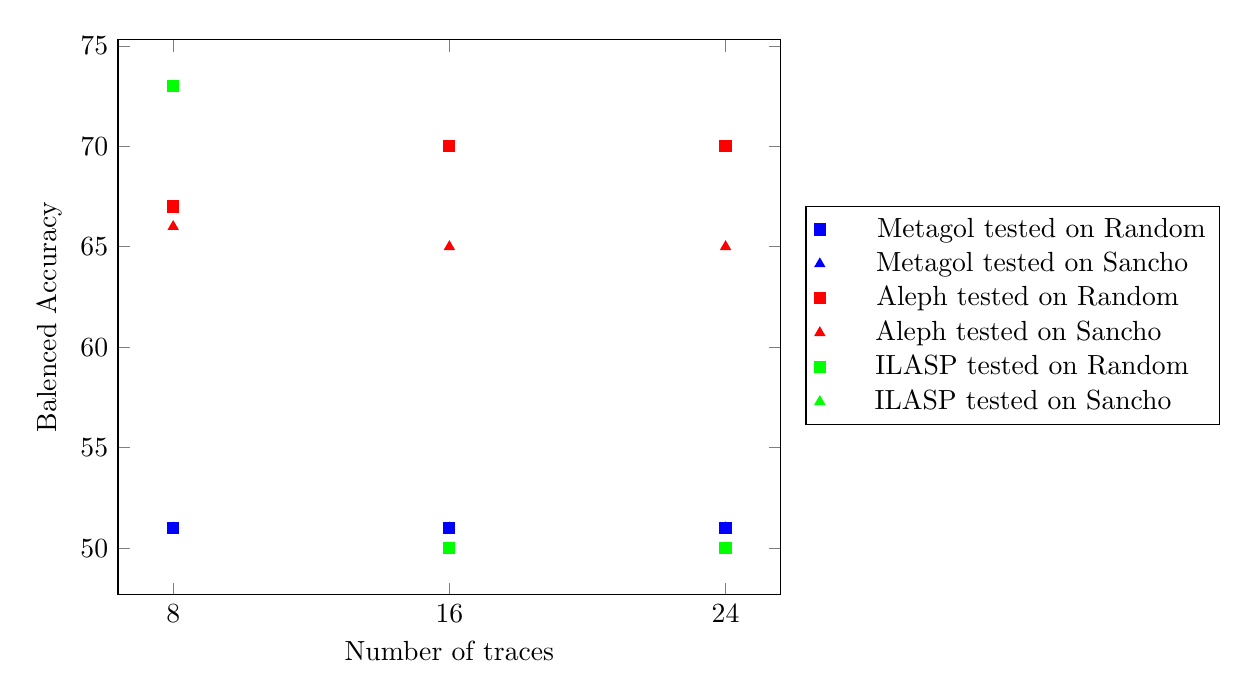
\begin{tikzpicture}
\begin{axis}[scatter/classes={
	a1={mark=square*,blue},%
	a2={mark=triangle*,blue},%
	b1={mark=square*,red},%
	b2={mark=triangle*,red},%
	c1={mark=square*,green},%
	c2={mark=triangle*,green}},
legend style={at={(1.35,0.7)},
	anchor=north},
xtick=data,
ylabel={Balenced Accuracy},
xlabel={Number of traces}]
\addplot[scatter,only marks,
scatter src=explicit symbolic] coordinates {
	(8,51)     	[a1]
	(8,51)     	[a2]
	(16,51)    	[a1]
	(16,51)    	[a2]
	(24,51)    	[a1]
	(24,51)		[a2]
	(8,67)		[b1]
	(8,66)		[b2]
	(16,70)		[b1]
	(16,65)		[b2]
	(24,70)		[b1]
	(24,65)		[b2]
	(8,73)		[c1]
	(8,73)		[c2]
	(16,50)		[c1]
	(16,50)		[c2]
	(24,50)		[c1]
	(24,50)		[c2]
};
\legend{\ \ \ \ \ Metagol tested on Random,\ \ \ Metagol tested on Sancho,\ \ Aleph tested on Random,Aleph tested on Sancho, \ \ \ ILASP tested on Random,\ ILASP tested on Sancho,d}
\end{axis}
\end{tikzpicture}
\\\\
When ILASP and Metagol have not had enough time to learn a predicate they output nothing. Both systems scale exponentially in time taken according to the size of the input. Whilst for Metagol it didn't have time even for the 8 traces ILASP ran out of time only on the 16 and 24 traces training sets. This had the effect for ILASP of a large drop in effectiveness. For 16 and 24 the default program consisting of just \textit{true} was used. This gave the balanced accuracy of 50 for each predicate. Metagol still managed to learn the simple predicates that it had managed on the 8 trace training set however did not increase at all in effectiveness over the rest of the experiment.

Unlike the other systems Aleph was consistently able to process the entire input since its method of learning is less computationally intense. When tested on the random traces Aleph did better with the increased number of traces. This was most likely due to the fact that more cases were encountered in the training data. Since Aleph usually ends up putting the cases it encounters straight into the program this simply meant there was a greater number of situations in the testing set that Aleph had seen before and was thus correctly able to classify. When tested on the optimal traces Aleph got worse. This is possibly due to the maximum size of Aleph programs taking effect. The clauses relevant to the optimal traces may be pushed out of the program by the vast number of clauses taken from the random gameplay examples.

If this experiment were to be conducted again much more enlightening results than these could be obtained by increasing the time given to each system to learn each predicate or even using a system with greater computational power to run the experiments. 



\chapter{Conclusions}
In this paper we have compared the ability of ILP systems to learn the rules of a game from observed gameplay in the IGGP framework on a range of training datasets. Primarily three ILP systems have been trained on random and intelligent gameplay as generated by the Sancho system. The generated hypotheses of the learners have been tested on random and intelligent gameplay from the same distributions as the training data. Differences in the effectiveness of the learned programs in correctly classifying legal and illegal gameplay were observed however there was not enough statistical significance in the results to disprove the null hypothesis. The systems were also trained on a mixture of optimal and random traces with similar results.

To test the significance of the size of the training dataset on the ability of the ILP systems to learn the systems were trained on varying numbers of game playouts. It was a training dataset of above 16 game traces had little effect on the ability to learn of the systems tested. 

\subsubsection{Limitations}

%\textbf{What is intelligence?} In this paper we use the concept of intelligence in relation to game traces without formally defining it. Future work could supply a framework with which we can define the intelligence of gameplay generated.


\textbf{ILP systems} In this paper we only test on three ILP systems, it is clear a more representative result could be obtained by testing on more systems. Techniques such as probabilistic\cite{Bellodi/Probablistic,Raedt/Probabalistic} and interactive\cite{Raedt/Interactive} learning are not used by any of the systems tested here. ILASP is the only system designed to handle noisy data\cite{MarkLaw/ILASP2i}, it would be interesting to try others with this approach\cite{Oblak/Noise,Evans/Noise}. The systems used also have many customisable settings for example Metagols metarules which have major implications for the programs learnt\cite{Cropper/Metarules}. Aleph has many different search methods on the hypothesis space many of which may yield better results than the default algorithm used in this paper.

\textbf{Generating traces} Whilst Sancho generates good examples of intelligent play it would be interesting to see traces generated by other general game playing methods\cite{Park/GGPAdvances,Kowalski/GGP}. For some games there exists a provably optimal set of moves in some cases such as for eight puzzle Sancho generates these moves (see section \ref{sec:sancho}) however it does not for all such games\cite{Schaeffer/Checkers}. Future research could compare the effects on the learned hypotheses when trained on optimal data. It may also be more insightful to look at the difference between human generated data and random or optimal.

\textbf{Other machine learning systems} There exists a huge variety of machine learning systems other than ILP. It is possible some of these may exhibit more of a bias toward one of the training sets. Testing a neural network or genetic algorithm based approach may provide insightful results.

\textbf{Intelligent verses random in other contexts} There are plenty of other domains other than game playing in which datasets can be considered intelligent or random. An example of this might be training a car to drive where you could train it on different quality levels of driving or training a facial recognition system on poor or high quality photos. These would prove an interesting area to study.

\textbf{How do humans compare} We have spent a lot of this paper investigating whether machines learn better on intelligent gameplay or random gameplay with the assumption that a human would learn better from watching another human play than random legal moves. Whilst in reality we might generally choose to watch a human playing when trying to learn a game rather than observing random legal moves it may not be the most effective way. Any real world example of this is almost always accompanied by additional information. For example humans would often have access to some description of the rules or someone explaining the edge cases that may not occur. It is hard to compare the how humans learn to how machines learn since the extra context a human is given around a game is so much greater than that of a machine which gets very little. It would be interesting to see how humans would fare in similar experiments to those in this paper. The experiment would have to include games unknown to the participant which preferably would not share too many common features with know games. Looking into this question would give new insights into the results of this paper. As with the similar question posed in this paper the experiment does not have clear predicted outcome.




\bibliography{project}
\bibliographystyle{plain}
\end{document}
